
\chapter{Thevenin Equivalent Circuits}

\section{Pre-lab Calculation}

\noindent

1) Determine an equation for the Thevenin equivalent voltage $V_{\rm th}$ and resistance $R_{\rm th}$ from the values $V_1, V_2, R_1, R_2, R_3$ for the circuit shown in Fig.~\ref{fig:thevenin}.
Hint:  Use the superposition principle.  Find the equivalent resistance by setting the voltage $V_1$ and $V_2$ to zero, i.e. shorting them in the circuit.  Then calculate two contributions to the Thevenin voltage, one with $V_1$ set to zero and one with $V_2$ set to zero.  The actual Thevenin voltage is the sum of these two contributions.  Play close attention to the polarity of $V_2$ as drawn, i.e. that a positive value of $V_2$ tends to make the voltage $V_{\rm a b}$ negative.

2) Compute $V_{\rm th}$, $R_{\rm th}$, and the short-circuit current $I_{\rm sc}$ for the particular values of $R_1$,$R_2$,$R_3$,$V_1$, and $V_2$ you will be using in the lab.

\begin{figure}[htbp]
\begin{center}
\begin{tabular}{c@{\hskip 2cm}c}
\begin{circuitikz}[line width=1pt]
\draw (0,0) to[battery1,bipoles/length=1.5cm,l=$V_1$] ++(0,2.0) coordinate(X) to[R,l=$R_2$,-*] ++(2.0,0);
\draw (X) to[R,l=$R_1$] ++(0,2.0) to[short,-*] ++ (2.0,0) coordinate(X) to[short,-o] ++ (1.0,0) node[right]{(a)};
\draw (X) to[battery1,bipoles/length=1.5cm, l=$V_2$] ++(0,-2.0) to[R,l=$R_3$] ++(0,-2.0) coordinate(X)
to[short,*-o] ++ (1.0,0) node[right]{(b)};
\draw(X) to[short] ++(-2.0,0);
\end{circuitikz} &
\begin{circuitikz}[line width=1pt]
\draw (0,0) coordinate(X) to[battery1,bipoles/length=1.5cm,l=$V_{\rm th}$] ++(0,2.0) to[R,l=$R_{\rm th}$,-*] ++(0,2.0)
to[short,-o] ++ (3.0,0) node[right]{(a)};
\draw(X) to[short,-o] ++ (3.0,0) node[right]{(b)};
\end{circuitikz} \\
(a) & (b) \\
\end{tabular}
\caption{The circuit (a) you will be building in lab and it's (b) Thevenin Equilvalent.}
\label{fig:thevenin}
\end{center}
\end{figure}

\section{Thevenin Equivalent Circuit}

Build the circuit in Fig.~\ref{fig:thevenin} using $R_1 = 3.3~\rm k\Omega$, $R_2 = 4.7~\rm k\Omega$, and $R_3 = 3.9~\rm k\Omega$.  Supply $V_1 = 10~\rm V$ and $V_2 = 5~\rm V$ using your two channel bench-top power supply.  In the diagram, the supplies are not referenced to ground or each other, so make certain that your supply is set to provide independent outputs and do not add any jumpers to ground.  Take careful note of the polarity of the supplies, so e.g. the negative (black) output of $V_1$ is connected to point (b) whereas the negative (black) output of $V_2$ is connected to point (a).

Use your Triplett 9007 as a voltmeter and the Mastech MS8624 as a current meter.
First measure the open circuit voltage $V_{\rm ab}$.  Next short the points (a) and (b) through your current meter.  These values should closely match the Thevenin voltage and short-circuit current which you have already calculated.  If not, you should check your work and find the discrepancy before proceeding.

Next you will measure the voltage across and current through a load resistor connected between the terminals at (a) and (b) to experimentally determine the IV curve for your circuit.  Recall from the previous lab that you measure the current by connecting your meter in series and the voltage by connecting your meter in parallel.  As before, use your Triplett 9007 as a voltmeter and the Mastech MS8624 as a current meter.

Make simultaneous current and voltage measurements for three different values of the load resistance $R = 470~{\rm Omega}, 1.2~\rm k\Omega, 4.7~\rm k\Omega.$



\section{Analysis}

{\bf Plot 1:}  To present your analysis you should produce a part like that of Fig.~\ref{fig:egthev}.  Your plot should show the Thevenin equivalent source IV curve for the circuit you built in lab.  You should also draw theoretical load IV curves for the three resistor values you used to make current and voltage.  Finally, you include data points for the five measurements you made.

\begin{figure}[htbp]
\begin{center}
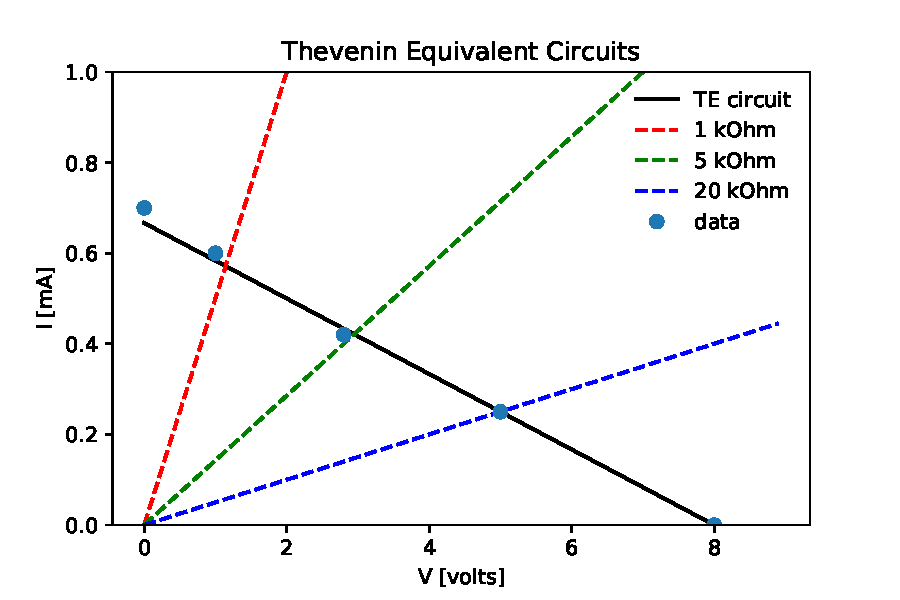
\includegraphics[width=0.75\textwidth]{figs/labs/thevenin/final.pdf} 
\caption{Using boolean masks to cut on variable $y$.}
\label{fig:egthev}
\end{center}
\end{figure}
